\documentclass{article}
\usepackage[utf8]{inputenc}
\usepackage{amssymb, amsmath, geometry, nopageno, xfrac, nicefrac, mathtools}
\usepackage{graphicx}
\graphicspath{ {./images/} }

\setlength{\textheight}{600pt}
\DeclarePairedDelimiter\abs{\lvert}{\rvert}%
\DeclarePairedDelimiter\norm{\lVert}{\rVert}%
\DeclareMathOperator{\im}{Im}
\DeclareMathOperator{\rank}{rank}
\DeclareMathOperator{\range}{range}
\DeclareMathOperator{\col}{col}
\DeclareMathOperator{\row}{row}
\DeclareMathOperator{\nullity}{nullity}
\DeclareMathOperator{\nullspace}{null}
\DeclareMathOperator{\spans}{span}
\DeclareMathOperator{\diag}{diag}
\DeclareMathOperator{\tr}{tr}
\DeclareMathOperator{\vect}{vec}
\DeclareMathOperator{\PProjection}{proj}
\DeclareMathOperator*{\argmin}{argmin} 


\newcommand{\F}{\mathbb{F}}
\newcommand{\real}{\mathbb{R}}
\newcommand{\C}{\mathbb{C}}
\newcommand{\linear}{\mathcal{L}}
\newcommand{\PP}{\mathcal{P}}
\newcommand{\R}{\mathcal{R}}
\newcommand{\M}{\mathcal{M}}
\newcommand{\U}{\mathcal{U}}
\newcommand{\V}{\mathcal{V}}
\newcommand{\W}{\mathcal{W}}
\newcommand\inner[2]{\langle #1, #2 \rangle}
\newcommand{\vct}{\mathbf}
\newcommand{\PProj}[2][]{\PProjection_{\vct{#1}}\vct{#2}}




\title{Linear Algebra Reference Sheet}
\author{By Danny Liu}
\date{}

\begin{document}
\maketitle

\section{Basic Knowledge}
A vector space is an Abelian group under vector addition with defined scalar multiplication over $\F$ \\
$v_1, v_2, ..., v_n$ is linearly independent when $c_1v_1 + c_2v_2 + \ldots + c_nv_n = 0$ has only the trivial solution\\
If $E$ is an elementary matrix, then $EA$ performs a row operation and $AE$ a column operation \\
$A \sim B$ if they represent the same linear operator under possibly different bases, written ${B = PAP^{-1}}$  

\subsection{Positive Definiteness}
A symmetric matrix $A$ is positive semi-definite if $x^TAx \geq 0 \mbox{ } \forall x \neq \boldsymbol{0} \iff Av = \lambda v \implies \lambda \geq 0 \\$
Positive definite matrices $x^TAx > 0$ are nonsingular and have positive diagonal elements \\
$f: \real^n \rightarrow \real$ is convex $\iff {\boldsymbol{H}_{\boldsymbol{f}} \mbox{ is positive semi-definite} \iff f(\boldsymbol{y}) \geq f(\boldsymbol{x}) + {\nabla f(\boldsymbol{x})}^T (\boldsymbol{y}-\boldsymbol{x}) \mbox{ }\forall \boldsymbol{x}, \boldsymbol{y} \in \real^n }$\\
Taylor expansion of $f$ at $\boldsymbol{z} \in [\boldsymbol{x}, \boldsymbol{y}]$ is $f(\boldsymbol{y}) =  f(\boldsymbol{x}) + {\nabla f(\boldsymbol{x})}^T (\boldsymbol{y}-\boldsymbol{x}) + \frac{1}{2}(\boldsymbol{y}-\boldsymbol{x})^TH_f(\boldsymbol{z})(\boldsymbol{y}-\boldsymbol{x})$

\subsection{Vectorization}
$\nabla_x x^TAx = \nabla_x (\sum_{i, j}x_i x_j A_{ij}) = (A + A^T)x$, $\nabla_x Ax = A$, $\nabla_x x^Ty = y$, $\nabla_x x^Tx = 2x$ \\
$\sum_i(\sigma(\theta^Tx^{(i)}) - y^{(i)})x^{(i)} = X^T(\sigma(X\theta) - y)$, $\nabla_\theta \sigma(X\theta) = \diag(\sigma^\prime (X\theta))X$ \\
$\nabla_x f = (\frac{\partial f}{\partial x_1}, \ldots , \frac{\partial f}{\partial x_n})^T$, $\boldsymbol{J}_{\boldsymbol{f}} = \begin{bmatrix} \frac{\partial \boldsymbol{f}}{\partial x_1} \ldots \frac{\partial \boldsymbol{f}}{\partial x_n} \end{bmatrix}$, $\boldsymbol{H}_{\boldsymbol{f}} = \boldsymbol{J}(\nabla_x f)^T = \nabla_x^2f(x)^T$

\section{Change of Basis}
Let $B = \{b_1, b_2, ..., b_n\}$ a basis for $\V$ over $\F$ and $T \in \linear(\V)$. Then \\
$\PP_{B} = \begin{bmatrix} [e_1]_B & [e_2]_B  \ldots  [e_n]_B \end{bmatrix}$ where $\PP_{B}(v) = [v]_B$ and $\PP_{B}^{-1} = \begin{bmatrix} b_1 & b_2  \ldots b_n \end{bmatrix}$ \\
$\M(T) = \begin{bmatrix} Te_1 & Te_2  \ldots  Te_n \end{bmatrix}$ and ${\M(T)} ^{-1} = \begin{bmatrix} T^{-1}e_1 & T^{-1}e_2  \ldots  T^{-1}e_n \end{bmatrix}$ \\
$[\M(T)]_B = \PP_B \M(T) \PP_B^{-1} = \PP_{BE}[\M(T)]_{EE}\PP_{EB} =  \begin{bmatrix} [Te_1]_B & [Te_2]_B  \ldots  [Te_n]_B \end{bmatrix}$

\section{Orthonormal Bases}
A list of vectors $(v_1, \ldots, v_m)$ is orthonormal if $\inner {v_i} {v_j} = 0$ for $i \neq j$ and $\norm {v_i} = 1$ \\
If $\{e_1, \ldots, e_n\}$ is an orthonormal basis for $\V$ and $v \in \V$, then $v = \inner{v}{e_1}e_1 + \ldots + \inner{v}{e_n}e_n$ \\
A matrix $Q$ is orthogonal if its columns and rows form orthonormal bases or if $Q^{-1} = Q^T$ \\
An orthogonal matrix can be thought of as a change of basis or a rotation to a new coordinate axes \\
Orthogonal operators preserve inner product and norm. $\inner{Tx}{Ty} = \inner{x}{y}$ and $\norm{Tv} = \norm{v}$

\subsection{Gram-Schmidt}
If $v_i$ are independent, then there exist orthonormal $e_i$ such that $\spans(v_1, \ldots, v_m) = \spans(e_1, \ldots, e_m)$ \\
$e_1 = \frac{v_1}{\norm {v_1}}$, $e_2 = \frac{v_2 - \inner{v_2}{e_1}e_1}{\norm{v_2 - \inner{v_2}{e_1}e_1}}$, $e_3 = \frac{v_3 -  \inner{v_3}{e_2}e_2- \inner{v_3}{e_1}e_1}{\norm{v_3 -  \inner{v_3}{e_2}e_2- \inner{v_3}{e_1}e_1}} \dots$

\section{Invertible Matrix Theorem}
Let $A$ be an $n \times n$ matrix that represents $T \in \linear(\V, \W)$. Note this implies $\dim \V = \dim \W$. Then \\
$A \mbox{ is invertible} \iff A^T \mbox{ is invertible} \iff \det(A) \neq 0 \iff \rank(A) = n \iff 0 \mbox{ is not an eigenvalue of } A \\ \iff \range T = \W \iff \ker T = \{ \boldsymbol{0} \} \iff T \mbox{ is injective} \iff T \mbox{ is surjective}$

\section{Determinant and Trace}
The determinant is a function from $n \times n$ matrices to $\F$ defined recursively by $\det A = a$ if $A = [a]$ \\ 
and $\det A = \sum_j (-1)^{1+j}a_{1j} \det A_{1j}$ otherwise where $A_{ij}$ denotes deleting the $i$th row and $j$th column \\
$\abs {\det A} \mbox{ scales volume of vector transformed by $A$ and is 0 when it is collapsed to a lower dimension}$ \\
If $A$ is triangular, then $\det A = \prod_i a_{ii}$ where $a_{ii}$ are the diagonal elements \\
Interchanging rows or columns, $\det A = - \det A$. Adding rows or columns $\det A = \det A$ \\
$\det A = \prod_i^n \lambda_i $, $\det (AB) = \det A \det B$, $\det (cA) = c^n \det A$, $\det A^{-1} = \frac{1}{\det A}$, $\det A = \det A^T$


\subsection{Characteristic Polynomial}
$\det(\lambda I - T) = p(\lambda) = (\lambda-\lambda_1)^{d_1} \ldots (\lambda-\lambda_m)^{d_m}$ where $d_i = \dim G(\lambda_i, T) = \dim (\nullspace (T- \lambda I)^{\dim \V})$ \\
If $p(\lambda) = \lambda^n + c_{n-1}\lambda^{n-1} + \ldots + c_1\lambda + c_0$, then $c_{n-1} = -\tr A$ and $c_0 = (-1)^n \det A$ \\
$p(T) = O$ and the zeros of $p(\lambda)$ are the eigenvalues of $T$
\subsection{Trace}
The trace is a function from $n \times n$ matrices to $\F$ defined by $\tr A = \sum_i a_{ii}$ \\
Trace and determinant are both invariant under similarity, so $\tr A =  \tr (PJP^{-1}) = \sum_i^n \lambda_i $ \\
$\tr (X^TY) = \sum_{i, j} X_{ij}Y_{ij} = \vect (X)^T \vect(Y) \approx \inner{X}{Y}$, $\tr (ABC) = \tr(CAB) = \tr(BCA)$ 

\section{Fundamental Theorem of Linear Algebra}
Every $m \times n$ real matrix $A$ contains four fundamental subspaces described by $A = U\Sigma V^T$ \\

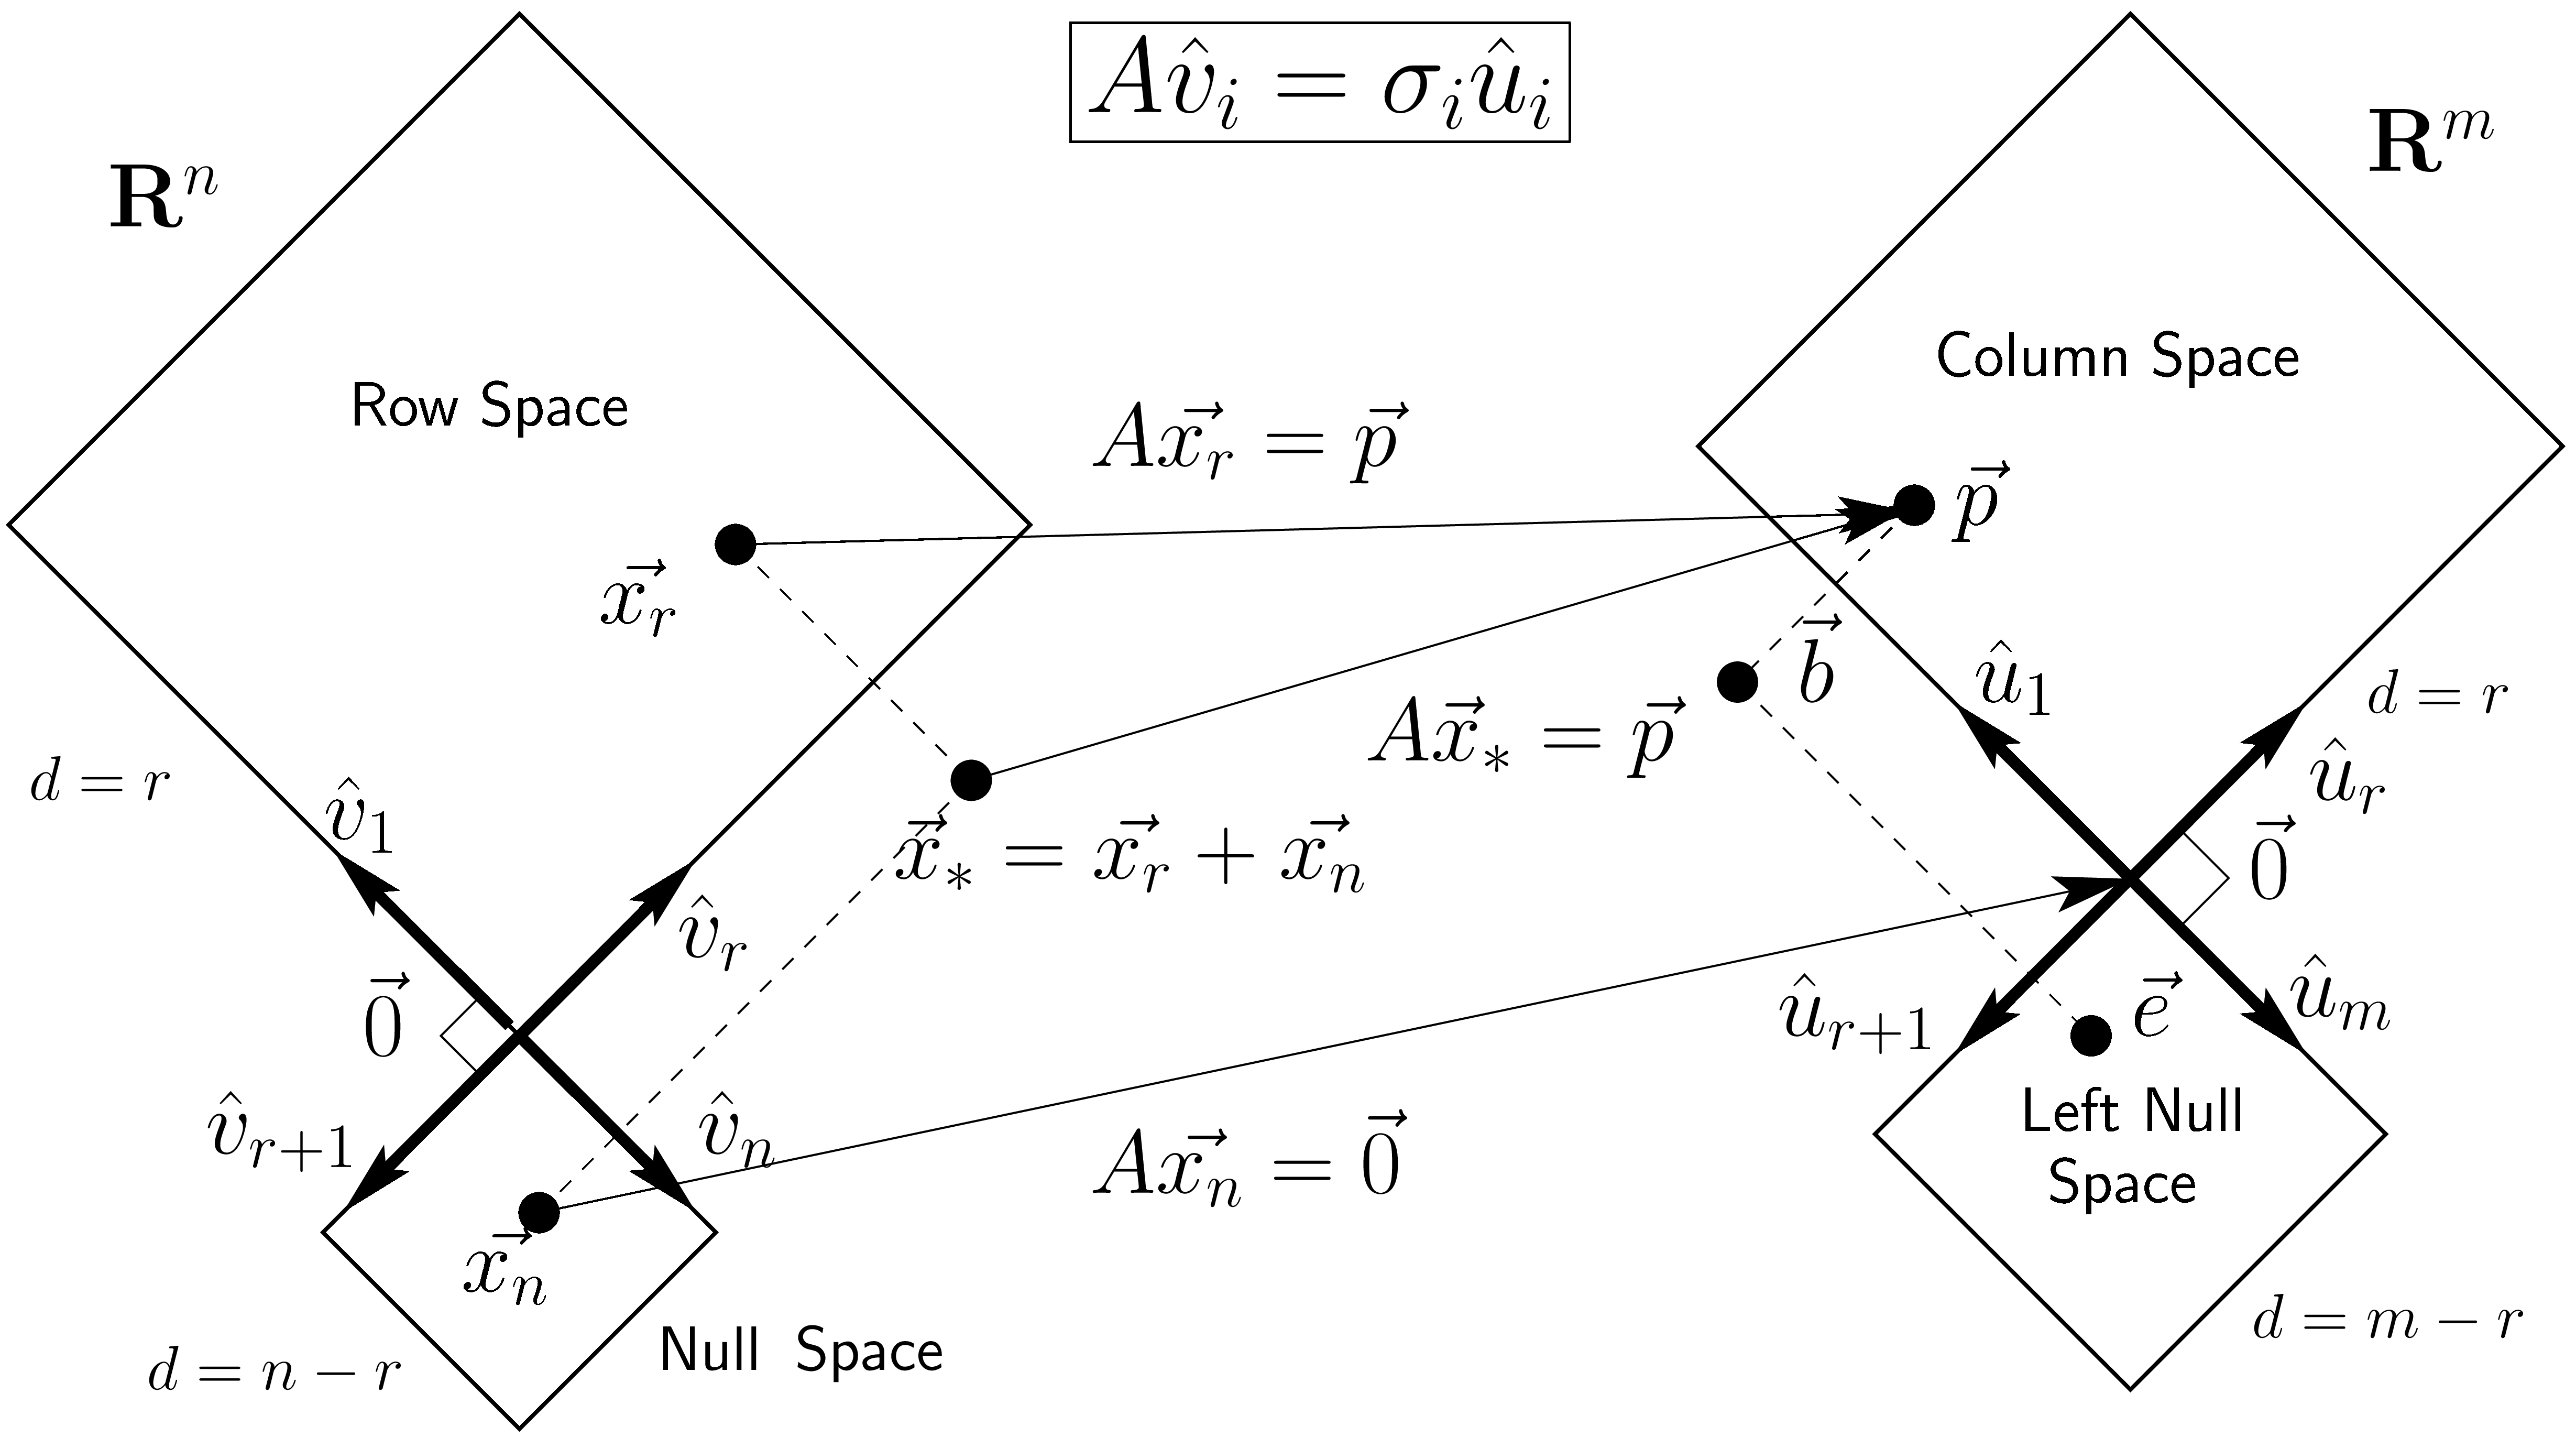
\includegraphics[width=8cm]{fund_thm.png} \\
This implies if $T \in \linear(\V, \W)$, then $\V = \row T \oplus \ker T$ and $\W = \row T^* \oplus \ker T^*$ \\
$x \mapsto Ax \mbox{ is one-to-one} \iff \ker A = \{\boldsymbol{0}\}$. $\col A = \im A = \range A = \row A^T$ \\
$A \begin{bmatrix} v_1 \ldots v_r \end{bmatrix} = \begin{bmatrix} u_1 \ldots u_r \end{bmatrix} \diag(\sigma_1, \dots, \sigma_r) \implies A = U_r\Sigma_r V_r^T = u_1\sigma_1 v_1^T + \ldots u_r\sigma_r v_r^T$

\section{Rank-Nullity Theorem}
${\mbox{Let } T \in \linear(\V, \W)\mbox{, then }\rank(T) + \nullity(T)= \dim V\mbox{. Equivalently, }\dim (\im T) + \dim (\ker T) = \dim V}$.

\section{Diagonalization}
Let $T \in \linear(\V)$ and $\{\lambda_1, \ldots, \lambda_m\}$ denote the distinct eigenvalues of $T$. Then \\
$T \mbox{ is diagonalizable} \iff \V \mbox{ has a basis consisting of eigenvectors of } T \iff {\dim G(\lambda_i, T) = \dim E(\lambda_i, T)} \\ \iff \V = E(\lambda_1, T) \oplus \dots \oplus E(\lambda_m, T) \iff \V = U_1 \oplus \dots \oplus U_n \mbox{ where each } U_i \mbox{ is invariant under } T$  \\
$A = PDP^{-1}$ where $P = \begin{bmatrix} v_1 & v_2 \ldots v_n\end{bmatrix}$ and $D = \diag(\lambda_1, \ldots, \lambda_n)$ \\
$D = [A]_B$ where $B$ is the basis consisting of eigenvectors of $A$ and $P^{-1} = P_{BE}$ 
\subsection{Spectral Theorem}
If $\V$ is a real inner-product space and $T \in \linear(\V)$, then $\V$ has an orthonormal basis consisting of eigenvectors of $T$ if and only if $T$ is self-adjoint (symmetric). \\
If $A$ is orthogonally diagonalizable, then $A^T = (PDP^{-1})^T = (P^{-1})^TDP^T = PDP^{-1} = A$ \\
${\mbox{If } A \mbox { is symmetric, then } (A-\lambda I)^2v = 0 \implies v^T(A-\lambda I)^2v = 0 \implies \norm{(A-\lambda I)v}^2 = 0 \implies Av = \lambda v}$

\section{Singular Value Decomposition}
Any real $m \times n$ matrix $A$ can be factored into $A = U \Sigma V^T$ where $U, V$ are orthogonal matrices whose columns are the orthonormal eigenvectors of $AA^T$ and $A^TA$ respecitvely and $\Sigma$ is the $m \times n$ diagonal matrix of the square roots of the nonzero eigenvalues values of $A^TA$.
\subsection{Key Insights}
Add rest of basis vectors $v_{r+1} \ldots v_n$ and $u_{r+1} \ldots u_n$ to $V_r$ and $U_r$ to make them orthogonal matrices \\
$A^TA = (AA^T)^T \succeq 0$, so they are orthogonally diagonalizable and have nonnegative eigenvalues \\
$A^TA = (U \Sigma V^T)^T U \Sigma V^T = V \Sigma^2 V^T, \mbox{ from which } V \mbox{ and } \Sigma \mbox{ can be implied by spectral decomposition}$ \\
When $A$ is square, the transformation can be viewed as a change of basis (rotation 1) $V^T$, a scaling in that intermediate basis $\Sigma$ and then another change of basis (rotation 2) $U$ \\
$A^T = (U \Sigma V^T)^T = V \Sigma^T U^T$ viewed as inverse rotation (2), same scaling and inverse rotation (1) \\
$A^{-1} = (U \Sigma V^T)^{-1} = (V^T)^{-1} \Sigma^{-1} U^{-1} = V \Sigma^{-1} U^T$. Inverse scaling, assuming that $A^{-1}$ exists.

\section{QR Decomposition}
$\mbox{Any }m \times n \mbox{ matrix }A\mbox{ with linearly independent columns can be factored into }A = QR\mbox{, where }Q \mbox{ is} \\ \mbox{an } m\times n \mbox{ matrix with orthonormal columns and } R \mbox{ is a nonsingular upper triangular matrix}$. \\
$A = \begin{bmatrix} u_1 & u_2 \ldots u_n\end{bmatrix} = \begin{bmatrix} q_1 & q_2 \ldots q_n\end{bmatrix} 
\begin{bmatrix} \inner{q_1}{u_1} & \inner{q_1}{u_2} & \ldots \\
0& \inner{q_2}{u_2} & \ldots \\
\vdots & \vdots & \ddots
\end{bmatrix}$ \\
If $A$ does not have linearly independent columns, then $R$ will be singular

\section{Triangular Matrices}
The inverse, product and sum of an upper (lower) triangular matrix is upper (lower) triangular \\
A triangular matrix is invertible if and only if the entires on its main diagonal are nonzero \\
${\M(T-\lambda I) \mbox{ is not invertible} \iff \lambda = d_i \mbox{ for some diagonal element } d_i \implies \mbox{eigenvalues on main diagonal}}$ \\
$\mbox{If }Ax = b\mbox{ where }A\mbox{ is lower triangular and nonsingular, then }x_1 = \sfrac{b_1}{a_{11}}\mbox{, ..., }x_n = \frac{b_n - \sum_{k=1}^{n-1}a_{nk}x_k}{a_{nn}}$ \\
Inverse can be computed by solving $A\begin{bmatrix} x_1 & x_2 \ldots x_n\end{bmatrix} = \begin{bmatrix} e_1 & e_2 \ldots e_n\end{bmatrix}$ column by column \\
$\mbox{If }A = LU,\mbox{ then let }Ux = y\mbox{ and solve }Ly = b\mbox{ via forward-substitution and }Ux=y\mbox{ by back-substitution}$

\subsection{LU Decomposition}
$\mbox{If }A\mbox{ is square and nonsingular, then }A = LU\mbox{ for unit lower triangular } L \mbox{ and upper triangular }U$ \\
Defining $E_{ij}$ to remove the $i$th row in the $j$th column, we have that $U = E_{n, n-1}\ldots E_{32} E_{n, 1}\ldots E_{21}A$ \\
$A = E_{21}^{-1} \ldots E_{n, 1}^{-1} E_{32}^{-1} \ldots E_{n, n-1}^{-1} U = LU$, where $E_{ij}$ has $-\frac{a_{ij}}{a_{jj}}$ at index $(i, j)$ \\
If $A$ is singular, then there exists $P$ such that the algorithm $PA = LU$ avoids dividing by zero

\subsection{LDU Decomposition}
If $A$ admits an LU decomposition, then $A = LDU$ for unit triangular $L$, $U$ and diagonal $D$ \\
Let $D = \diag (u_{11}, \ldots, u_{nn})$ and $U_1 = \frac{U}{\vect D}$, then $A = LDU_1$ as $L$ is already unit triangular

\subsection{Cholesky Decomposition}
If $A$ is real positive definite, then $A = LL^T$ for a lower triangular $L$ with positive diagonal entries. \\
$A \succ 0 \implies A = LDU = A^T = (LDU)^T = U^TDL^T = LDL^T = (LD^{\frac{1}{2}})(D^{\frac{1}{2}} L^T) = L_1L_1^T$ \\
Since $L$ is nonsingular, let $y = L^Tx$. Then $y^TDy = x^TLDLx = x^TAx > 0 \implies D \succ 0$ \\
Once existence proved, find $L$ by $l_{jj} = \sqrt{a_{jj} - \sum_{k=1}^{j-1}l_{jk}^2}$ and $l_{ij} = \frac{1}{l_{jj}}(a_{ij} - \sum_{k=1}^{j-1}l_{ik}l_{jk})$ for $i > j$

\section{Inner Products}
$z = a + bi$, $\abs z^2 =  z \bar{z} = (a+bi)(a-bi) = a^2 + b^2$, $\inner u v  = \overline{\inner v u}$, ${\norm v}^2 = \inner v v$ \\
Euclidean inner product over $\C$ becomes $\inner {(u_1, \ldots, u_n)} {(v_1, \ldots, v_n)} = u_1 \overline{v}_1 + \ldots + u_n \overline{v}_n$ \\
If $\inner u v = 0$, then ${\norm {u + v}}^2 = {\norm u }^2 + {\norm v}^2$ (Pythagorean) \\
$\abs {\inner u v} \leq \norm u \norm v$ (Cauchy-Schwartz) and $\norm{u + v} \leq \norm u + \norm v$ (Triangle)

\subsection{Adjoints}
The adjoint of $T \in \linear(\V, \W)$ is $T^* \in \linear(\W, \V)$ such that $\inner{Tv}{w} = \inner{v}{T^*w}$ for all $v \in \V, w \in \W$ \\
$\mbox{If } B \mbox { is an orthonormal basis for }\V, \mbox{ then }[T^*]_B = [T]_B^* \mbox{ where } [T]_B^* \mbox{ is the conjugate transpose of } [T]_B$

\subsection{Orthogonal Projections}
$\PProj[v] {u} = \frac{\inner{u}{v}}{\inner{v}{v}} v = \frac{\norm u \norm v \cos \theta}{{\norm v}^2}v = \frac{(u_1v_1 + \ldots u_nv_n)\hat{v}}{\norm v}  = \norm u \cos \theta \hat{v}$ \\
The orthogonal complement of $\U \subseteq \V$ is $\U^{\perp} = \{v \in \V \mid \inner{v}{u} = 0 \mbox{ }\forall u \in \U \}$ \\
$\V^{\perp} = \{\boldsymbol{0}\}$ and $\U^{\perp}$ is always a subspace of $\V$. If $\U \subseteq \V$ is a subsapce, then $\V = \U \oplus \U^{\perp}$ \\
Let $\U \subseteq \V$ be a subspace. The orthogonal projection of $\V$ onto $\U$ is the operator $P_{\U}$ where if $v = u + w$ where $u \in \U$ and $w \in \U^{\perp}$, then $P_{\U}(v) = u$ \\
If $T \in \linear(\V)$, then $U\mbox{ is invariant under }T \iff P_UTP_U = TP_U \iff U^\perp \mbox{ is invariant under }T^*$ \\
Given a subspace $\U$ of $\V$ and a vector $v \in V$, then $P_{\U}(v) \coloneqq \argmin\limits_{u \in U} \norm{u - v}$ 


\subsection{Riesz Representation Theorem}
If $\varphi: \V \rightarrow \F$ is a linear form, then there exists a unique $u \in \V$ such that $\varphi(v) = \inner v u$ for all $v \in \V$

\end{document}

